% Latex template: mahmoud.s.fahmy@students.kasralainy.edu.eg
% For more details: https://www.sharelatex.com/learn/Beamer

\documentclass{beamer}					  % Document class

\usepackage[portuguese]{babel}			  % Set language
\usepackage[utf8x]{inputenc}			  % Set encoding

\mode<presentation> {					  % Set options
  \usetheme{default}					    % Set theme
  \usecolortheme{default} 				% Set colors
  \usefonttheme{default}  				% Set font theme
  \setbeamertemplate{caption}[numbered]	% Set caption to be numbered
}

\setbeamertemplate{navigation symbols}{}
\setbeamertemplate{footline}[frame number]
\setbeamercovered{transparent}

% Uncomment this to have the outline at the beginning of each section highlighted.
%\AtBeginSection[]
%{
%  \begin{frame}{Outline}
%    \tableofcontents[currentsection]
%  \end{frame}
%}

\usepackage{graphicx}					% For including figures
\usepackage{booktabs}					% For table rules
\usepackage{hyperref}					% For cross-referencing
\usepackage{caption}                    % Allows more control over captions in figs and tables

\title{Revisão de Atividades da FAC}	% Presentation title
%\author{Author One}					% Presentation author
\institute{LNLS.DAC.FAC}				% Author affiliation
\date{2023-11-17 -- 2023-12-12}			% Today's date	


\begin{document}



\begin{frame}
  \titlepage
  \href{https://github.com/lnls-fac/doc-review-dac-fac}{\beamergotobutton{Link para o repo github desta apresentação: https://github.com/lnls-fac/doc-review-dac-fac}}
  \href{https://www.overleaf.com/read/sbdjxtzfchrm}{\beamergotobutton{Link para o projeto overleaf destas notas}}
\end{frame}

\begin{frame}{Outline}
  \tableofcontents
\end{frame}



\section{Estudos com o DELTA52}

\begin{frame}{DELTA52 - Caracterização e Correção}
    \begin{figure}[H]
    		\centering
            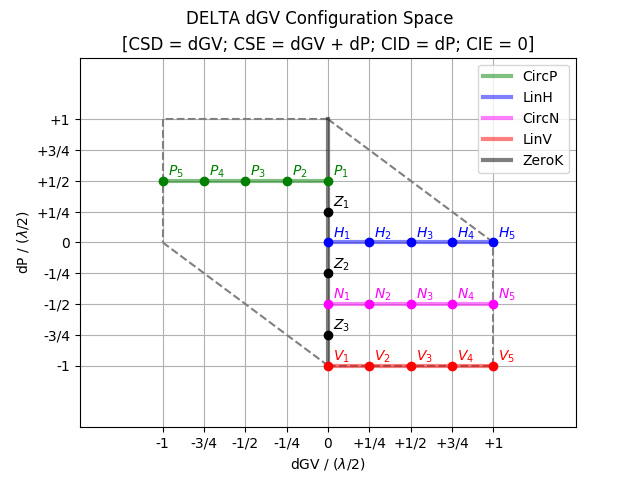
\includegraphics[width=.8\textwidth]{2023-12-12/figures/id-delta-dgv-config-space.png}
            \caption{Espaço de configuração do DELTA}
            \label{fig:delta-config-space}
    \end{figure}
\end{frame}

\begin{frame}{DELTA52 - Caracterização e Correção}
    \begin{itemize}
    		\item Movimentação do DELTA provoca a) distorções de órbita, b) mudança de acomplamento, c) distorção das funções beta, d) mudança da abertura dinâmica, tempo de vida, tc.
            \item Todos estes efeitos afetam a matriz resposta de órbita.
            \item correção local com pares de CHs, CVs, QSs, trims QFB, QDB1 e QDB2.
    \end{itemize}
    \begin{figure}[H]
        	\centering
            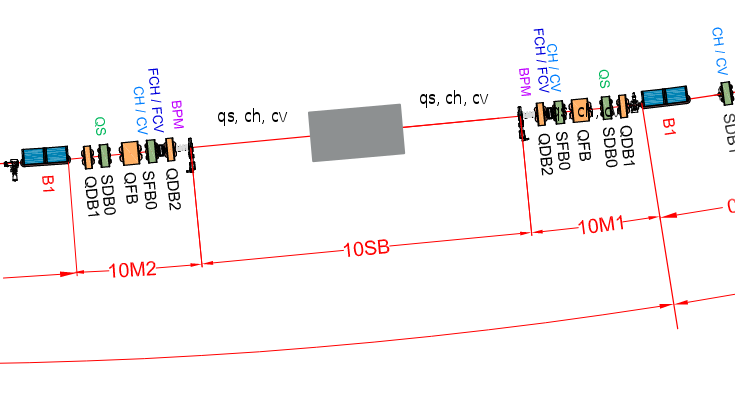
\includegraphics[width=0.6\textwidth]{2023-12-12/figures/si-10sb-2.png}
            \caption{\small{8 botões: 2 CHs, 2 CVs, 1 QS, QFB1, QFB, QDB2}}
            \label{fig:bba}
    \end{figure}
\end{frame}


\begin{frame}{DELTA52 - Caracterização e Correção}
    \begin{itemize}
    		\item Corretoras fitadas (iteração 0)
    \end{itemize}
    \begin{figure}[H]
        	\centering
            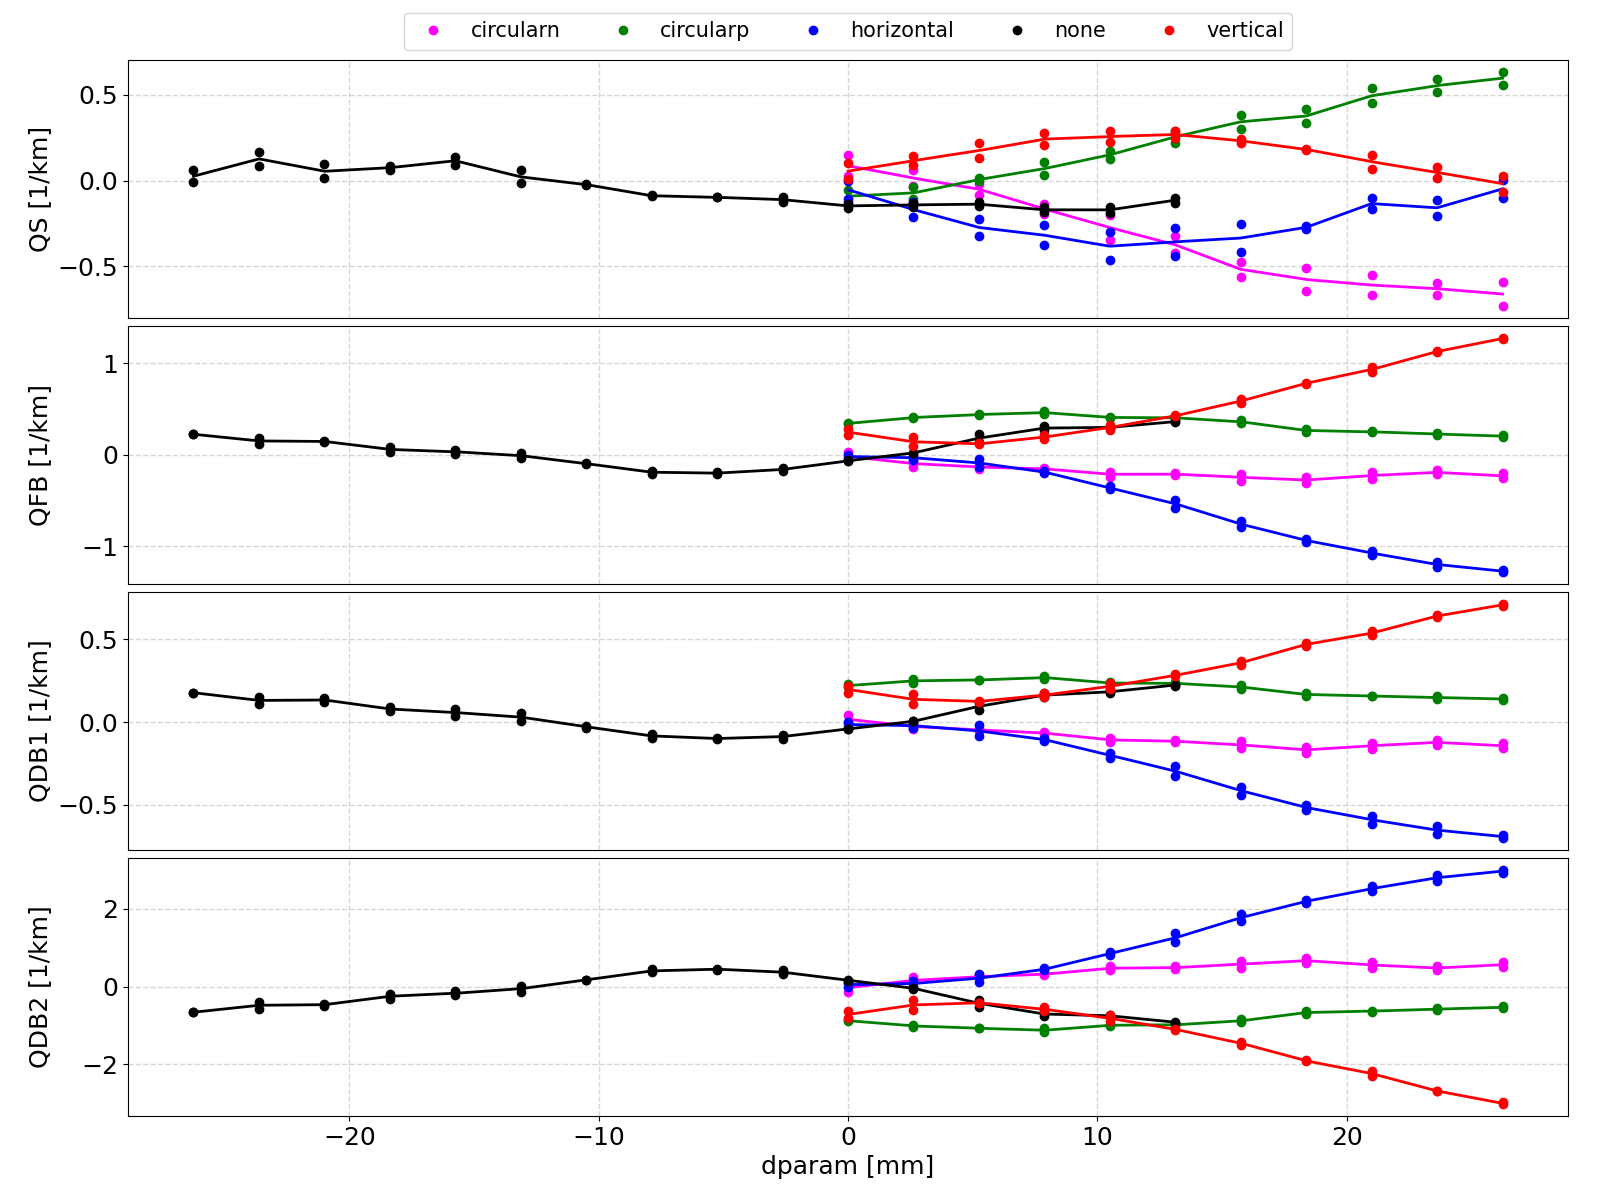
\includegraphics[width=0.8\textwidth]{2023-12-12/figures/knobs-before.png}
            % \caption{\small{No correction}}
            \label{fig:bba}
    \end{figure} 
\end{frame}


\begin{frame}{DELTA52 - Caracterização e Correção}
    \begin{itemize}
    		\item Corretoras fitadas (iteração 1 de QS)
    \end{itemize}
    \begin{figure}[H]
        	\centering
            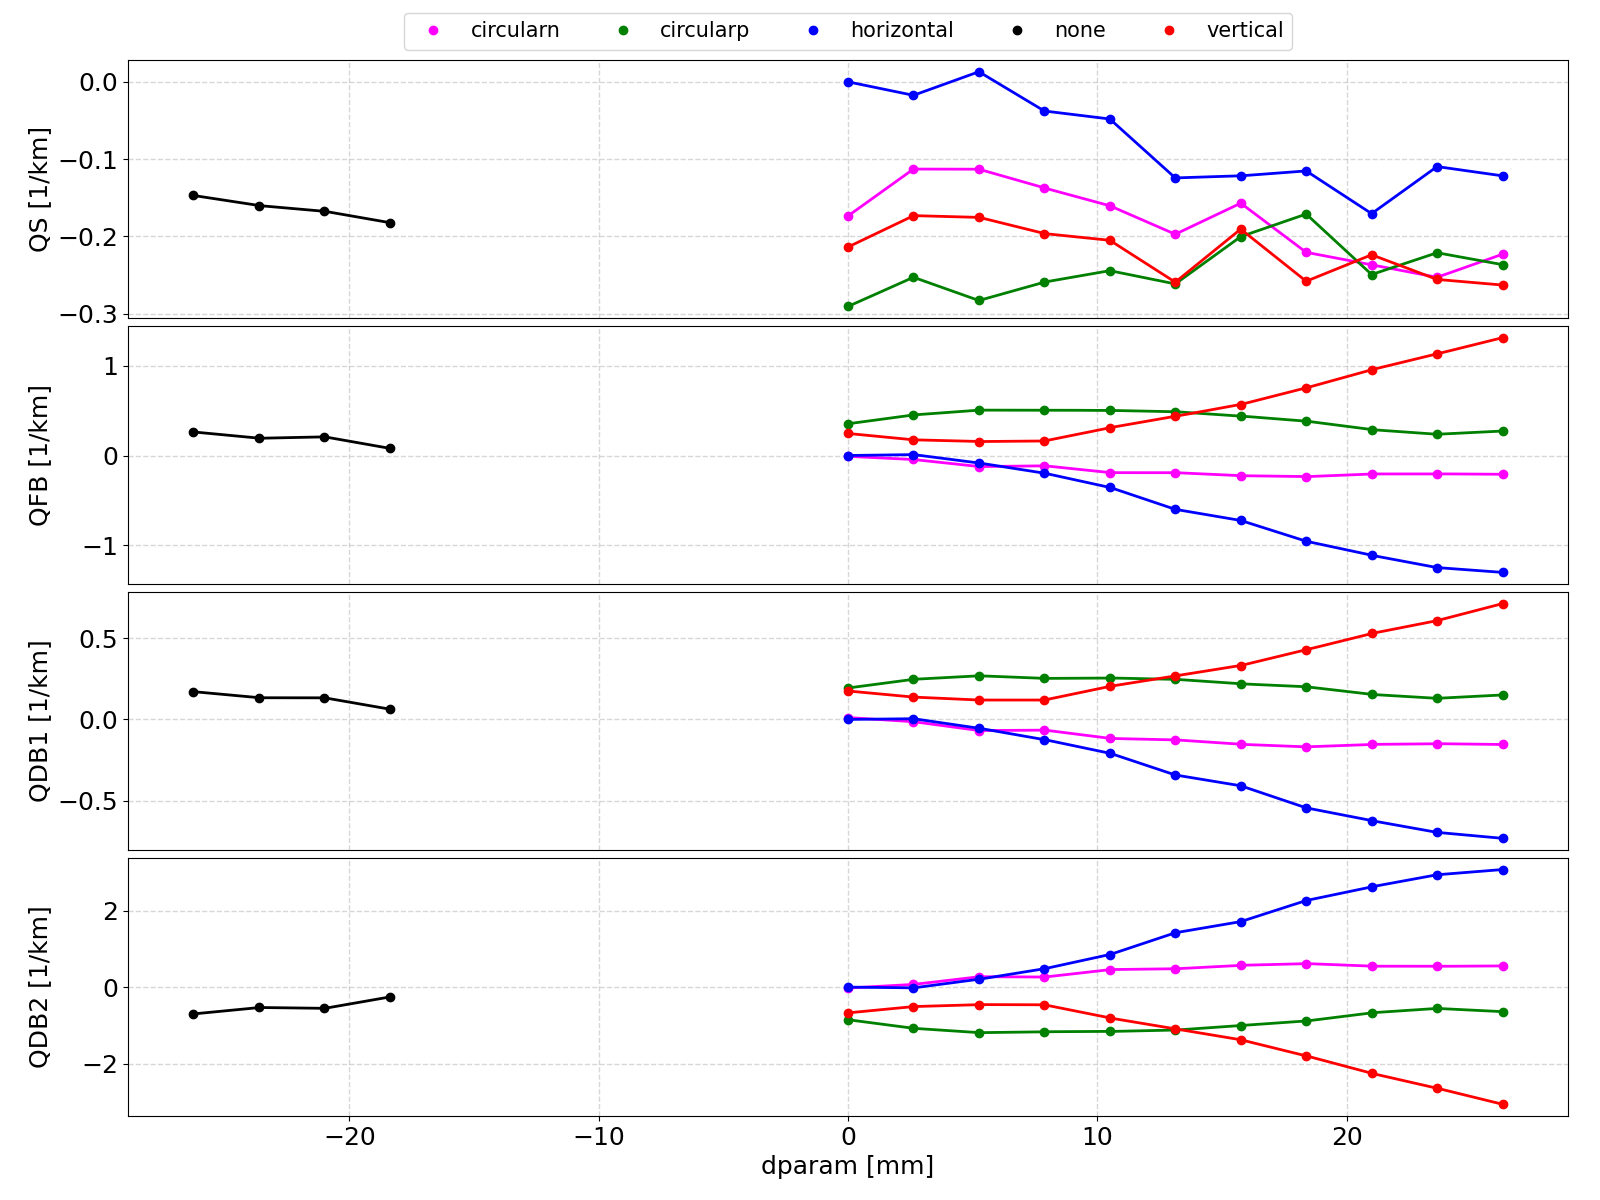
\includegraphics[width=0.8\textwidth]{2023-12-12/figures/knobs-after.png}
            % \caption{\small{No correction}}
            \label{fig:bba}
    \end{figure} 
\end{frame}


\begin{frame}{DELTA52 - Caracterização e Correção}
    \begin{itemize}
    		\item Efeitos da correção no acoplamento e emitância vertical
    \end{itemize}
    \begin{figure}[H]
        	\centering
            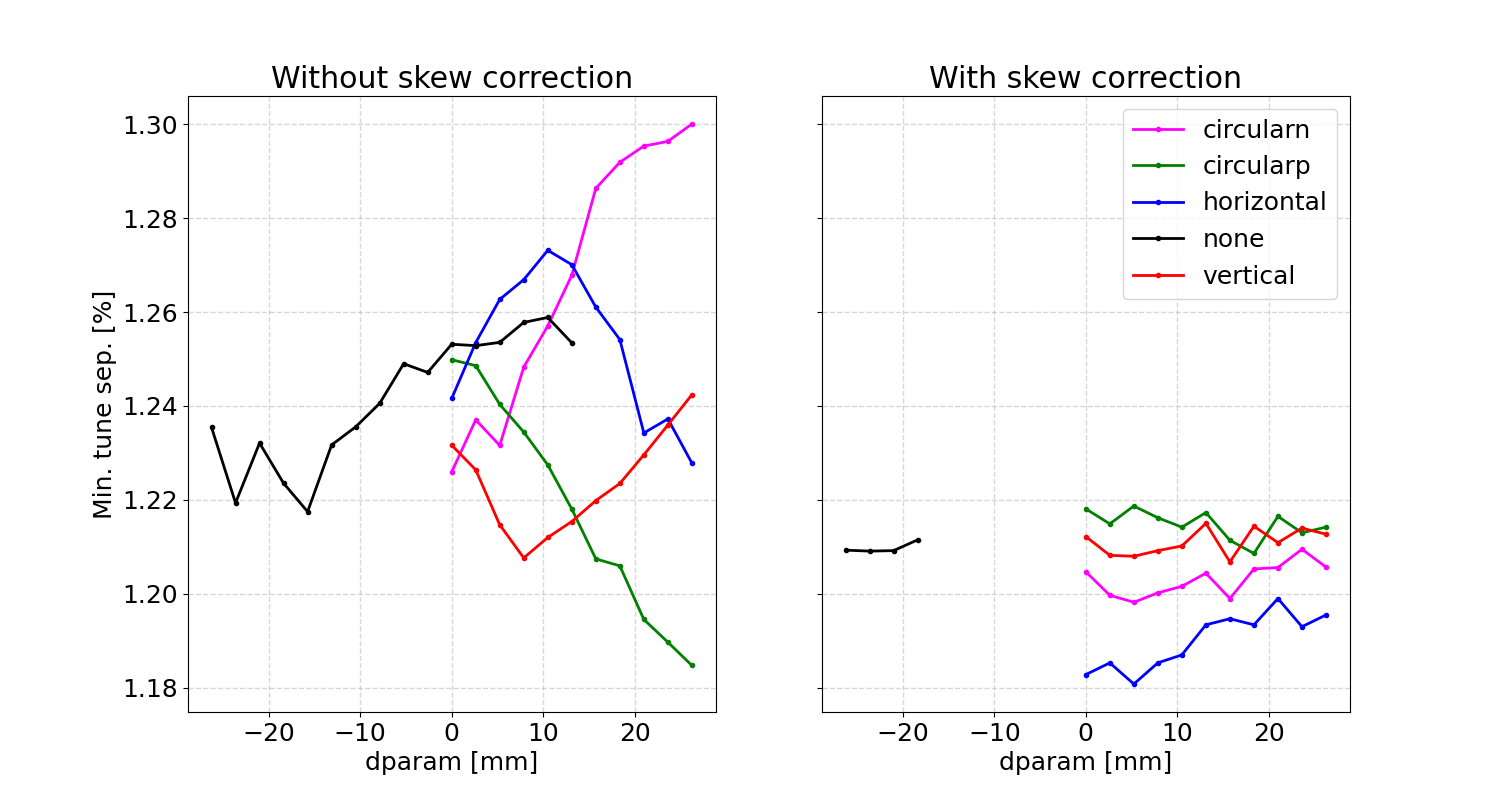
\includegraphics[height=3.5cm, width=9cm]{2023-12-12/figures/coupling.png}\\ 
            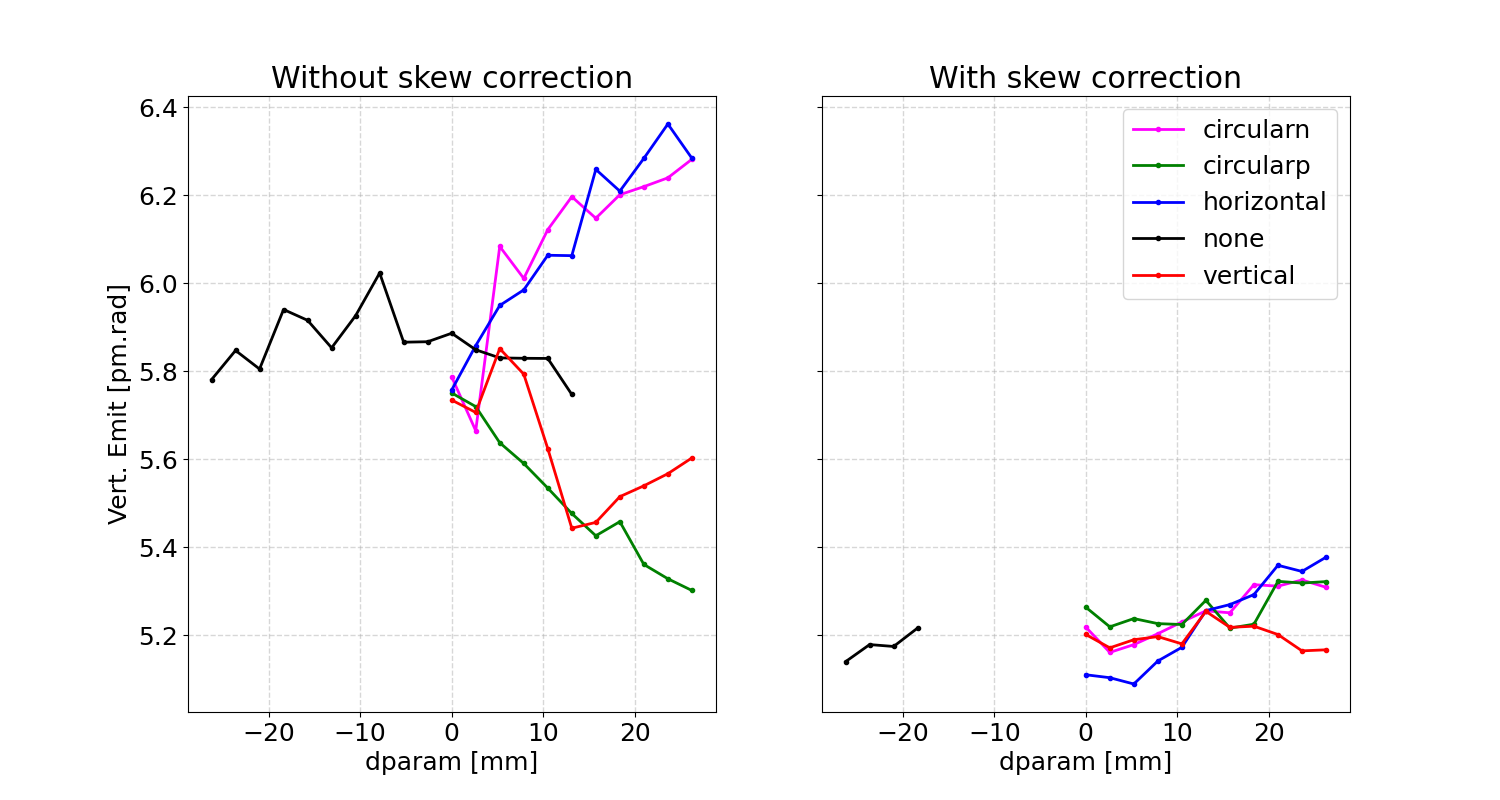
\includegraphics[height=3.5cm, width=9cm]{2023-12-12/figures/Vertical_emmitance.png}
            % \caption{\small{No correction}}
            \label{fig:bba}
    \end{figure} 
\end{frame}


\begin{frame}{DELTA52 - Caracterização e Correção}
    \begin{itemize}
    		\item Distorção de órbita e fitting de CHs e CVs
    \end{itemize}
    \begin{figure}[H]
        	\centering
            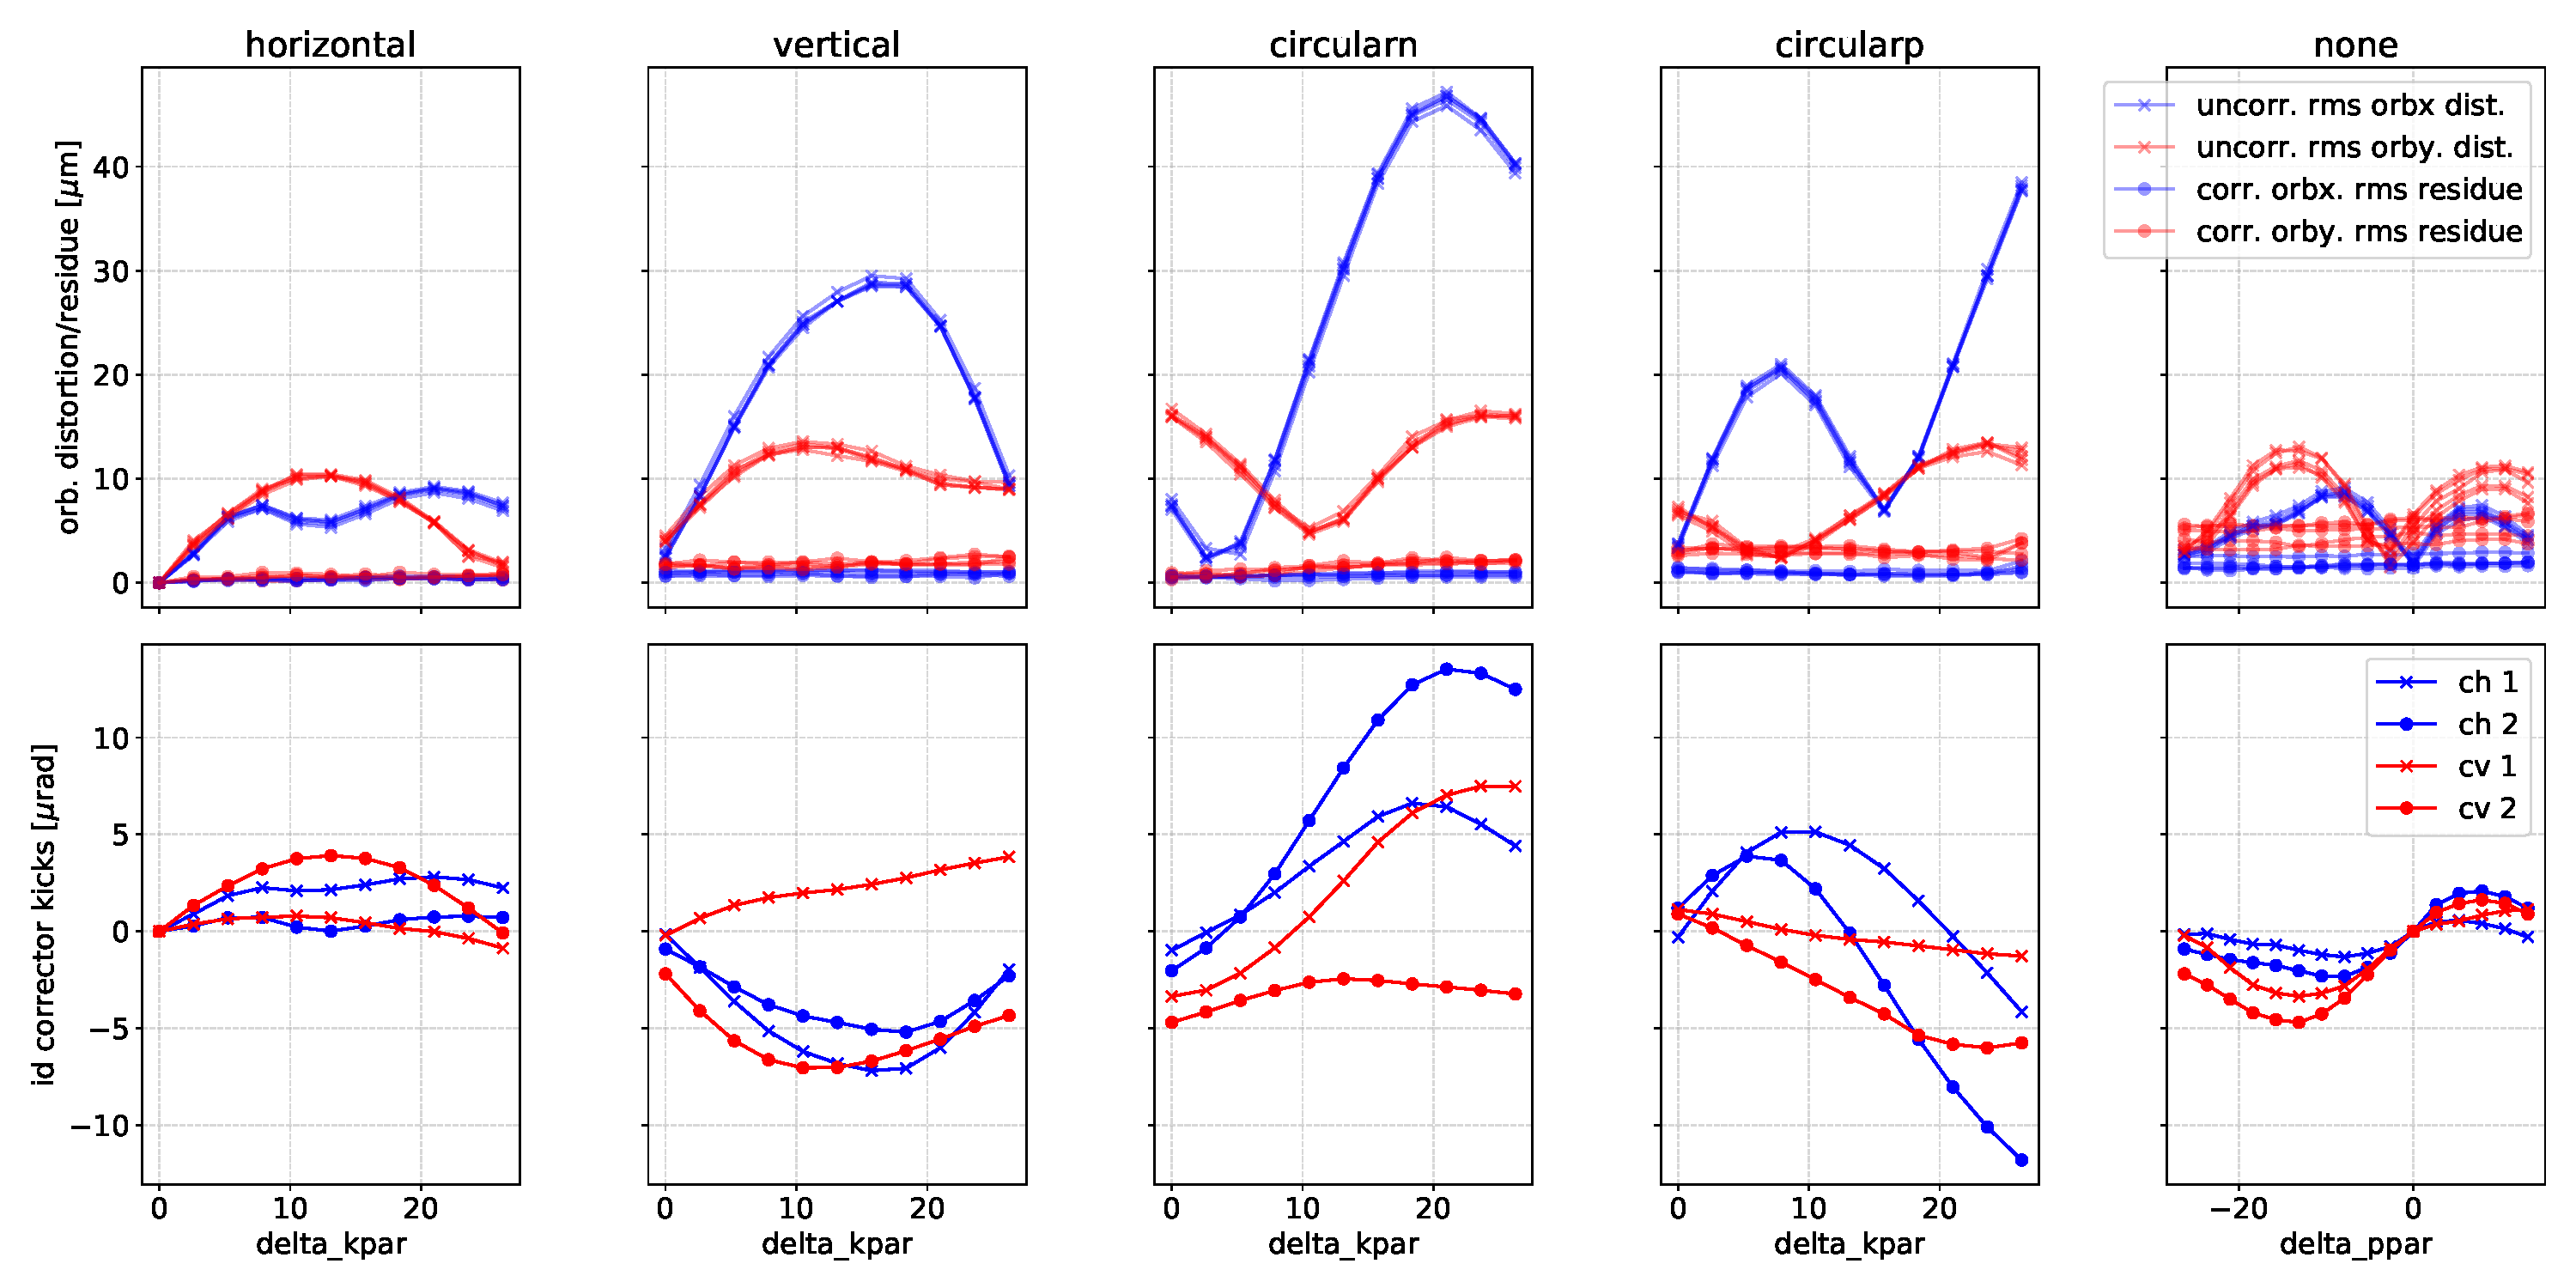
\includegraphics[width=0.9\textwidth]{2023-12-12/figures/orbcorr_ff.pdf}
            % \caption{\small{No correction}}
            \label{fig:bba}
    \end{figure} 
\end{frame}

\begin{frame}{DELTA52 - Feedforward}
    \scriptsize{\begin{itemize}
    		\item As tabelas de feedforward para QS, CH e CV estão medidas e implementadas
            \item O loop está rodando a 10 Hz desde 2023-12-11 com a configuração $delta52\_ref$
            \item A SABIÁ agora tem controle sobre as movimentações step do DELTA52.
            \item FF de QDB1, QFB e QDB2 ?
    \end{itemize}}
    \begin{figure}[H]
        	\centering
            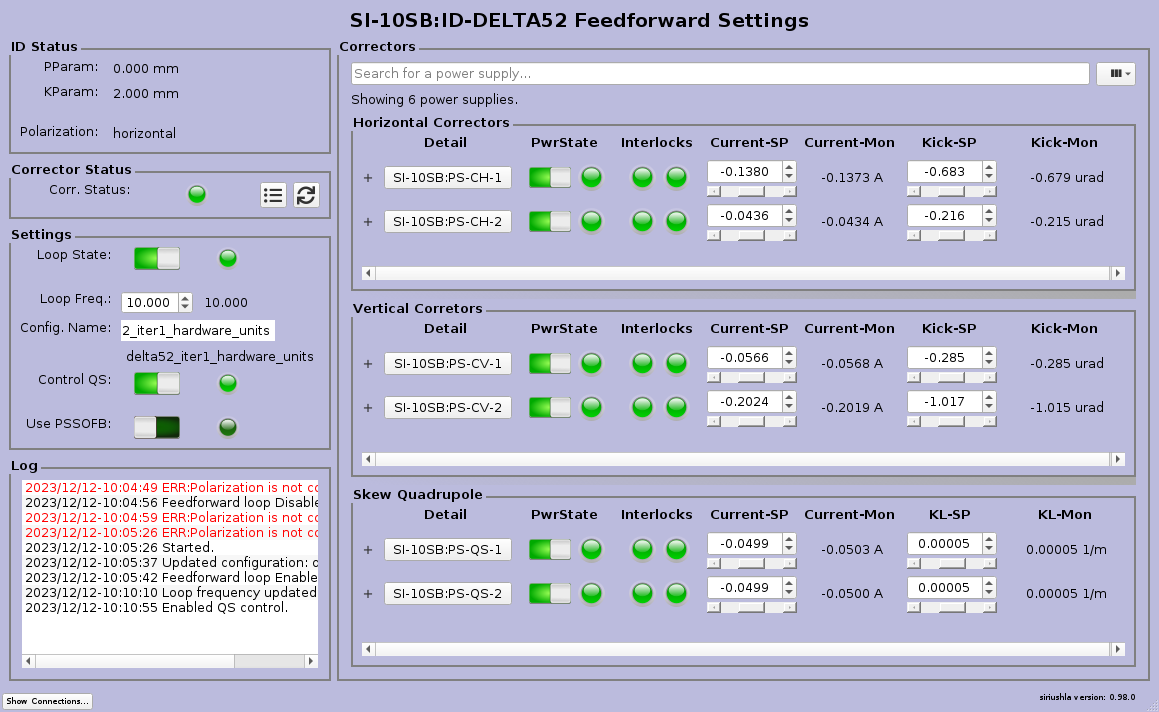
\includegraphics[width=0.8\textwidth]{2023-12-12/figures/idff.png}
            % \caption{\small{No correction}}
            \label{fig:bba}
    \end{figure} 
\end{frame}



\section{Reotimização das bobinas de compensação do NLK}

\begin{frame}{NLK - Reotimização}
    \scriptsize{\begin{itemize}
    		\item \href{https://ais-eng-srv-ta.cnpem.br/Olog/\#20923_4}{\beamergotobutton{Estudo de máquina em 2023-11-20}}
            \item Horizontal orb std (um): 23 (no opt), 7.7 (opt no interf),  5.5 (opt interf)
    \end{itemize}}
    \begin{figure}[H]
        	\centering
            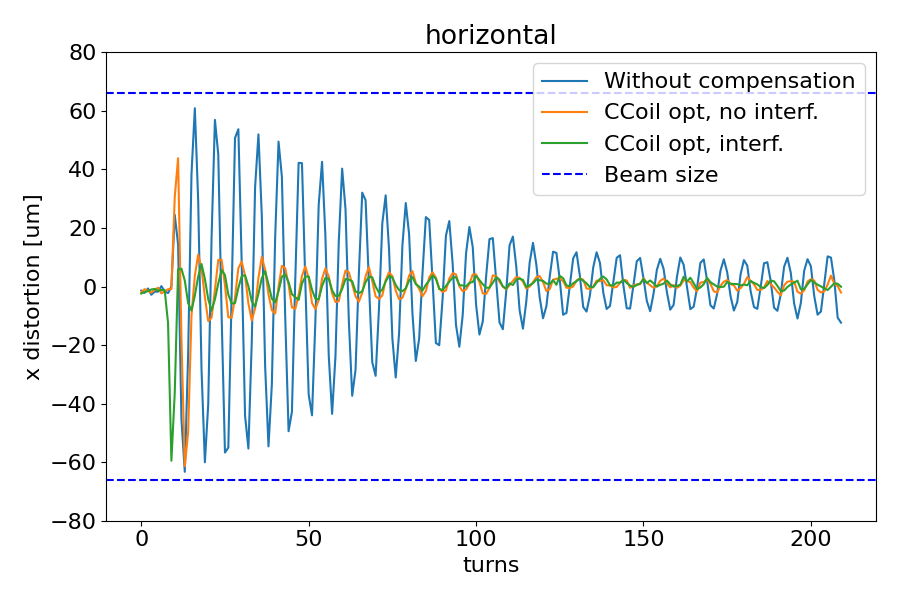
\includegraphics[width=0.8\textwidth]{2023-12-12/figures/horizontal_nlk_distortion_interference.png}
            % \caption{horizontal STD (um): 23 (no opt), 7.7 (opt no interf),  5.5 (opt interf)}
            \label{fig:bba}
    \end{figure} 
\end{frame}

\begin{frame}{NLK - Reotimização}
    \scriptsize{\begin{itemize}
    		\item \href{https://ais-eng-srv-ta.cnpem.br/Olog/\#20923_4}{\beamergotobutton{Estudo de máquina em 2023-11-20}}
            \item vertical orb std (um): 4.5 (no opt), 1.9 (opt no interf),  1.4 (opt interf)
    \end{itemize}}
    \begin{figure}[H]
        	\centering
            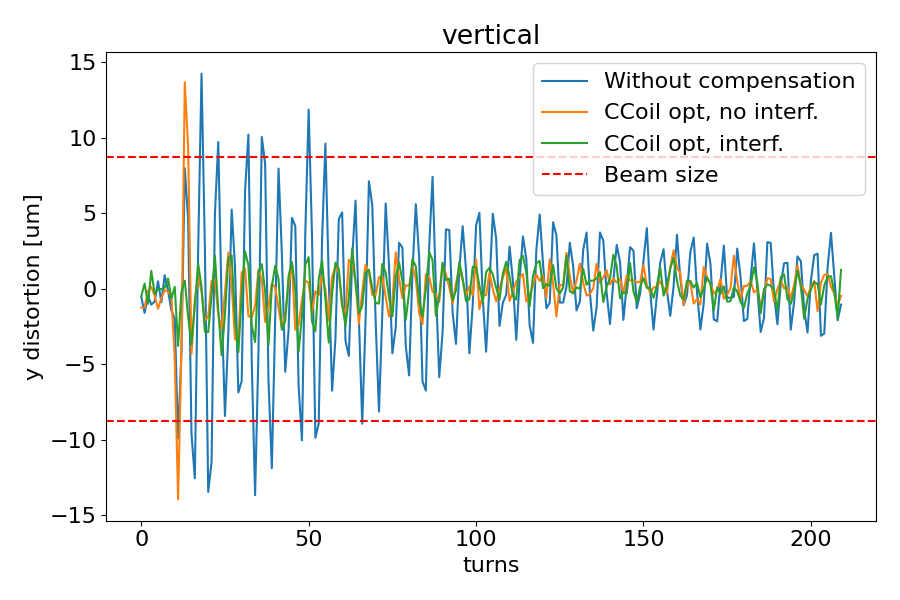
\includegraphics[width=0.8\textwidth]{2023-12-12/figures/vertical_nlk_distortion_interference.png}
            % \caption{vertical STD (um): 4.5 (no opt), 1.9 (opt no interf),  1.4 (opt interf)}
            \label{fig:bba}
    \end{figure} 
\end{frame}

\section{References}


\end{document}
